\documentclass[Rapport/Rapport_main.tex]{subfiles}
\begin{document}
\subsection{Logical View}
Det logiske view omhandler funktionaliteten af systemet, som leveres til brugeren. Systemets funktionalitet, struktur og adfærd beskrives ved brug af applikationsmodeller, heri klasse- og tilstandsdiagrammer. Der gennemgås de samme distributioner som i det forrige afsnit. \\\\
Klassediagrammerne er struktureret efter MVVM-arkitekturen, som illustreres i figur \ref{fig:MVVM_arch}. Tilstandsmaskinerne viser hvordan komponenterne interagerer med hinanden og deres relationer. 
\begin{figure}[H]
    \centering
    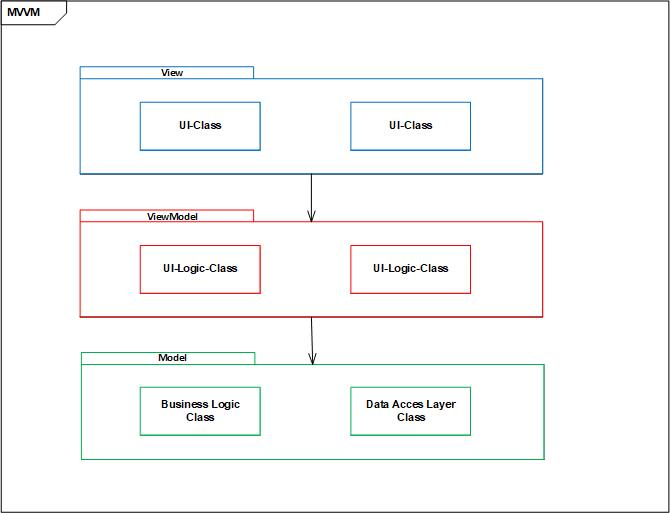
\includegraphics[width=\textwidth]{Rapport/Arkitektur/4+1/Logical/graphics/MVVMsketch.jpg}
    \caption{MVVM arkitektur}
    \label{fig:MVVM_arch}
\end{figure}
\noindent Arkitekturen for MVVM definerer, at ViewModeller ikke skal have nogen relation til View'et, som indeholder de grafiske elementer for systemet og er framework bestemt med hensyn til WPF. (Hermed kan man også genbruge ens ViewModeller, hvis man skifter framework). Det skal dog stadigvæk være muligt at skifte views, samtidigt med at ingen relation mellem View og ViewModel skabes. Til dette oprettes klassen ApplicationViewModel. Alle ViewModeller anvender denne klasse til at kunne skifte View.  

\subsubsection{Oprettelse af brugerprofil}
Systemet giver brugeren to muligheder ved programstart: Login eller tilmeldelse. Når et af de to krav er opfyldt, navigeres til selve programmet. HeaderbarView er brugerens mulighed for at navigere til andre views - den indeholder en navigationssti til næsten alle views i systemet. Brugerinformationerne gemmes i databasen, og kan fremover bruges til at logge ind med.  
\begin{figure}[H]
    \centering
    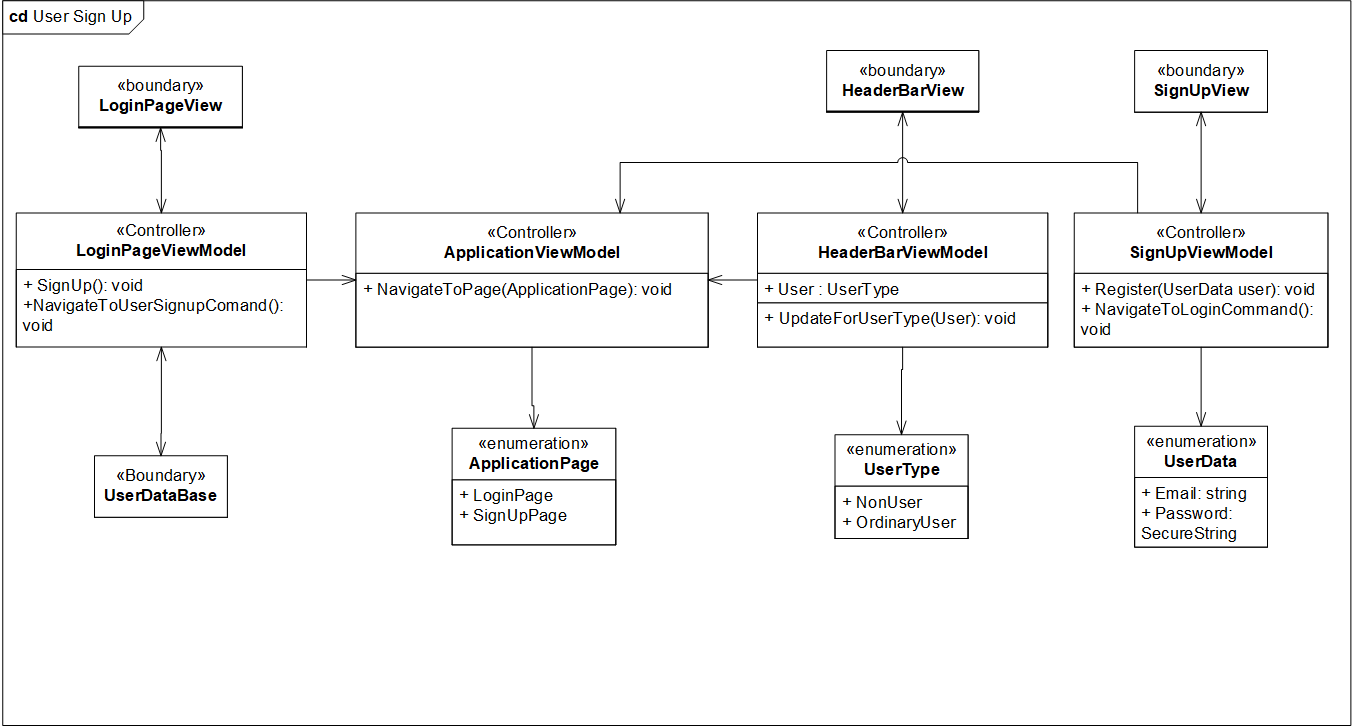
\includegraphics[width=\textwidth]{Arkitektur/Softwarearkitektur/User_Signup/graphics/UserSignUpCD.png}
    \caption{Klassediagram for oprettelse af bruger profil. }
    \label{fig:UserSignUpCD}
\end{figure}
\begin{figure}[H]
    \centering
    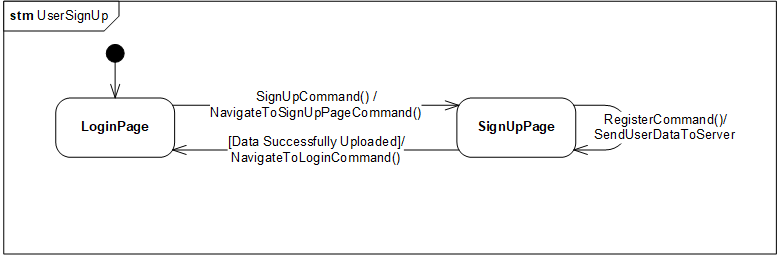
\includegraphics[width=\textwidth]{Arkitektur/Softwarearkitektur/User_Signup/graphics/UserSignUpSTM.png}
    \caption{Tilstandsdiagram for oprettelse af bruger profil. }
    \label{fig:UserSignUpSTM}
\end{figure}


\subsubsection{Oprettelse af bilprofil}
Hvis en bruger er registreret som udlejer, skal systemet give brugeren rettigheder til at oprette en bilprofil. Brugeren kan navigere til vinduet gennem HeaderBarView. Bilprofilen gemmes i databasen, og vil herefter vises i applikations udlejningskatolog.
\begin{figure}[H]
    \centering
    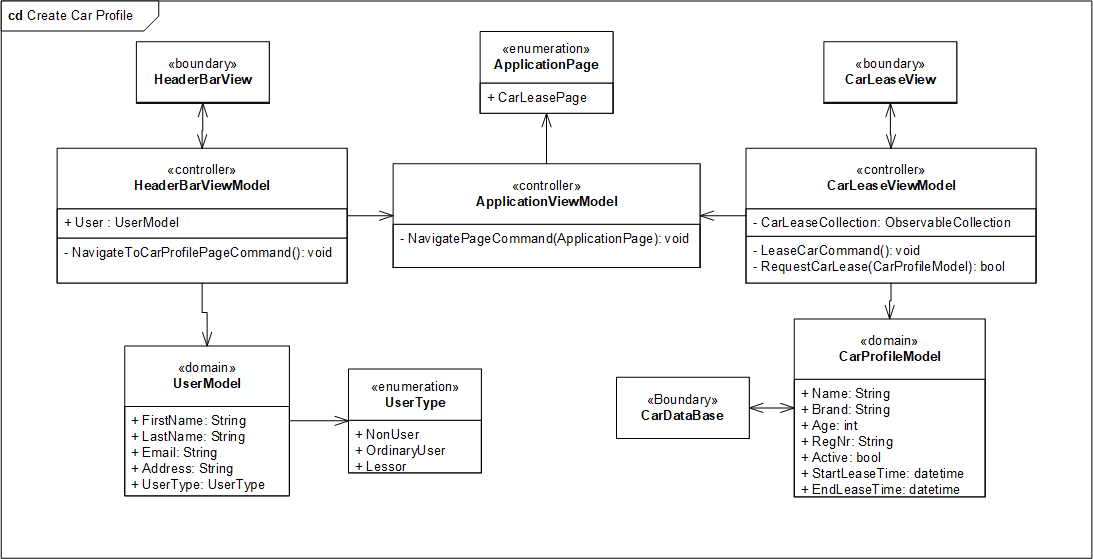
\includegraphics[width=1\textwidth]{Arkitektur/Softwarearkitektur/Car_registration/graphics/RegisterCarProfileCD.png}
    \caption{Her ses klassediagrammet for tilføjelse af bil til en brugerprofil. }
    \label{fig:RegisterCarProfileCD}
\end{figure}

\begin{figure}[H]
    \centering
    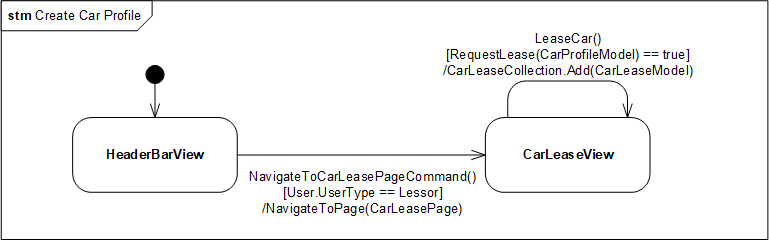
\includegraphics[width=1\textwidth]{Arkitektur/Softwarearkitektur/Car_registration/graphics/RegisterCarProfileSTM.png}
    \caption{Her ses tilstandsdiagram for tilføjelse af bil til en brugerprofil. }
    \label{fig:RegisterCarProfileSTM}
\end{figure}

\subsubsection{Søgning}
Brugeren navigerer til søgningssiden og angiver kriterier for biludlejningen (tidsinterval, bilmærke, lokation mv.). Systemet vil løbende hente bilprofiler fra databasen, der passer til brugerens kriterier. 
\begin{figure}[H]
    \centering
    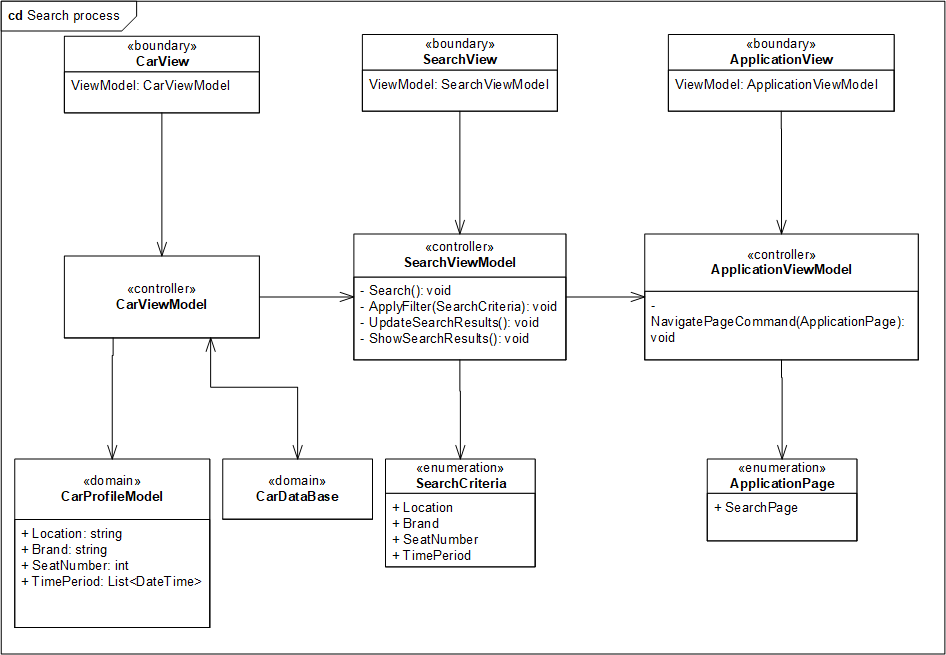
\includegraphics[width=1\textwidth]{Arkitektur/Softwarearkitektur/Searching/graphics/SearchProcessCD.png}
    \caption{Klassediagram for søgning efter biler til leje. }
    \label{fig:SearchProcessCD}
\end{figure}
\begin{figure}[H]
    \centering
    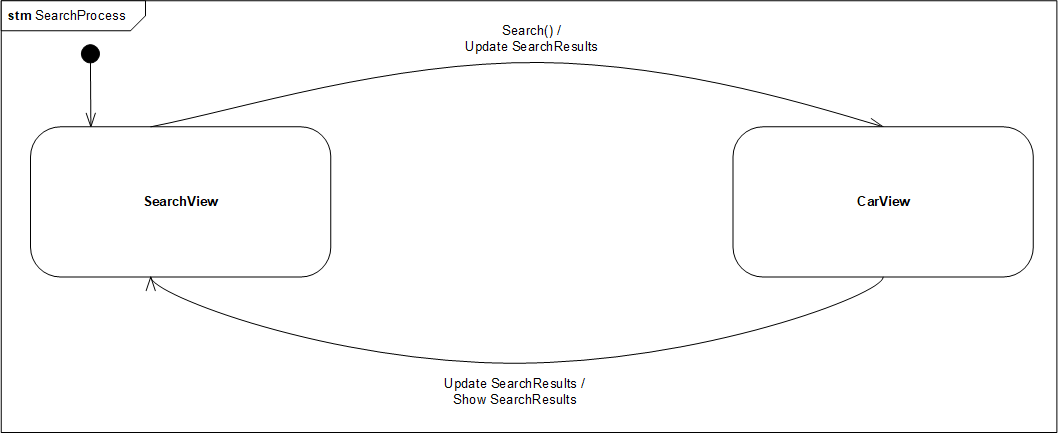
\includegraphics[width=1\textwidth]{Arkitektur/Softwarearkitektur/Searching/graphics/SearchProcessSTM.png}
    \caption{Tilstandsdiagram for søgning efter biler til leje. }
    \label{fig:SearchProcessSTM}
\end{figure}

\subsubsection{Håndtering af udlejningsproces}
Brugeren har nu fundet den bilprofil, som ønskes at lejes. Der navigeres til et vindue, hvor han kan sende en besked til udlejeren. Udlejeren vil nu modtage en besked, som kan findes i NotifikationView'et, som findes i Headerbaren. Hvis brugeren vælger en besked, navigeres der til et MessageView, som viser det fulde indhold af beskeden. Udlejeren kan enten godkende eller afvise anmodningen. Hvis anmodningen godkendes, udleveres udlejeres oplysninger til brugeren. 
\begin{figure}[H]
    \centering
    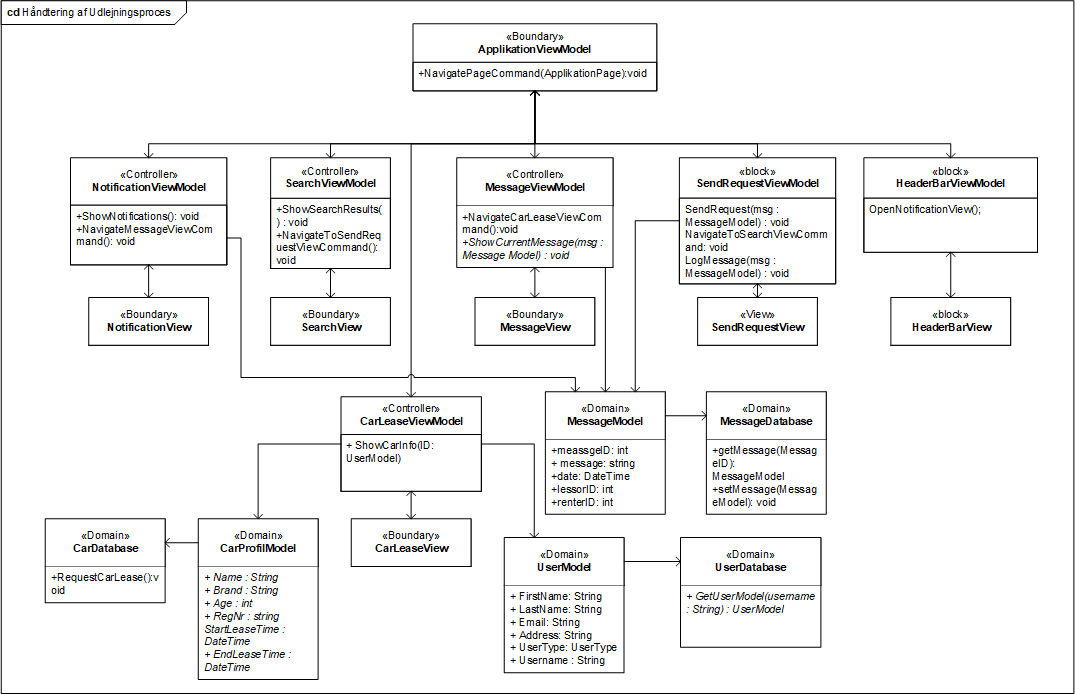
\includegraphics[width=1\textwidth]{Arkitektur/Softwarearkitektur/Leasing/graphics/Leasing_processCD.png}
    \caption{Klassediagram for håndtering af udlejningsprocessen.}
    \label{fig:Leasing_processCD}
\end{figure}

\begin{figure}[H]
    \centering
    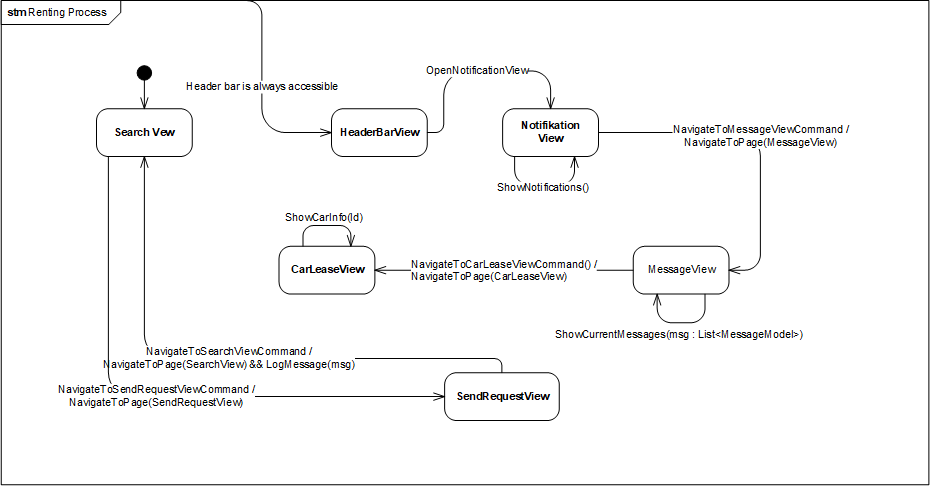
\includegraphics[width=1\textwidth]{Arkitektur/Softwarearkitektur/Leasing/graphics/Leasing_processSTM.png}
    \caption{Tilstandsdiagram for håndtering af udleningsprocessen. }
    \label{fig:Leasing_processSTM}
\end{figure}
\end{document}